\chapter{Go Endgames Using Neural Networks}
\label{ch:AlphaGo}
\epigraph{
  Creativity involves breaking out of established patterns in order to look at things in a different way.
}{Edward de Bono}
As of~today, over 20 years have passed since \Mueller's work.
\emph{DeepMind}, a~London-based AI start-up recently acquired by Google, has developed the strongest computer Go program so far:
\emph{AlphaGo}.

\begin{quotation} \noindent
  The game of~Go has long been viewed as~the most challenging of~classic games for artificial intelligence owing to its enormous search space and the difficulty of~evaluating board positions and moves.
\end{quotation}

\note{
  This chapter is based on~the article ``Mastering the game of Go with deep neural networks and tree search''~(\cite{Silver2016mastering}), which documents the internals of~AlphaGo.

  For more details, also consult my presentations on AlphaGo given at:
\begin{itemize}
  \item Spring School of Combinatorics 2016 (Charles University in~Prague): \\
    \href{http://www.slideshare.net/KarelHa1/mastering-the-game-of-go-with-deep-neural-networks-and-tree-search-presentation}
    {\tt http://www.slideshare.net/KarelHa1/mastering-the\\-game-of-go-with-deep-neural-networks-and-tree\\-search-presentation}

  \item Optimization Seminar (Charles University in~Prague) \\
    \href{http://www.slideshare.net/KarelHa1/alphago-mastering-the-game-of-go-with-deep-neural-networks-and-tree-search}
    {\tt http://www.slideshare.net/KarelHa1/alphago\\-mastering-the-game-of-go-with-deep-neural\\-networks-and-tree-search}

  \item Distributed Computing group (ETH \Zurich) \\
    \href{http://www.slideshare.net/KarelHa1/alphago-for-disco-group-of-eth-zurich}
    {\tt http://www.slideshare.net/KarelHa1/alphago\\-for-disco-group-of-eth-zurich}
\end{itemize}
}

\section{Game-Tree Search}
\epigraph{
  There are more possible positions in~Go than there are atoms in~the universe.
  That makes Go a~googol [$10^{100}$] times more complex than chess.
}{\href{https://deepmind.com/alpha-go.html}{Google DeepMind}}
Optimal value~$v^*(s)$ determines the~outcome of~the game from every board position $s$ under perfect play by~all players.
This value can be computed by~recursively traversing the~search tree containing approximately $b^d$ possible sequences of moves, where $b$ is the breadth of~game (number of legal moves per position) and $d$ is its depth (game length).

In~the case of~chess, that is $b \approx 35$ and $d \approx 80$, whereas Go has $b \approx 250$ and $d \approx 150$.
This amounts to a~terrifying overnumerousness: there are more Go positions than atoms in the observable Universe.
Therefore, exhaustive search is deemed intractable.

How to handle the size~of the game tree? For the$\dots$
\begin{itemize}
  \item $\dots$breadth: we train a~neural network to~select moves.
  \item $\dots$depth: we train a~neural network to~evaluate the current position.
  \item $\dots$tree traverse: we use Monte Carlo tree search method.
\end{itemize}

\textbf{Monte Carlo tree search} (MCTS) is a~Monte Carlo heuristic of~the classical tree search.
However, instead of traversing the entire game tree, the MCTS selects the~most promising moves, expanding the search tree based on~random sampling.

In~each iteration, the game is played-out to~the very end by~choosing moves at~random.
The final outcome of~each playout is then used to~weight the nodes in~the game tree accordingly.
Thus, better nodes are more likely to be chosen in future playouts.

\begin{figure}[H]
  \centering
  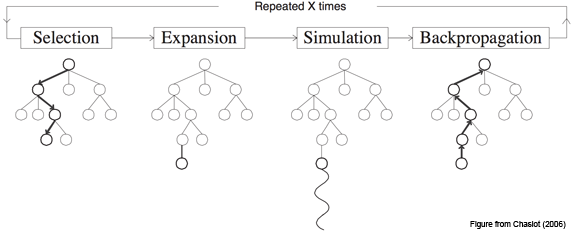
\includegraphics[width=.6\textwidth]{../img/MCTS.png}
  \caption{The scheme of~MCTS}
  \label{fig:MCTS}
\end{figure}

\section{Neural networks}

Inspired by biological neural networks, an~artificial neural network (ANN) is a~network of~interconnected nodes that make up a~model.
ANNs can be defined as~statistical learning models that are used to approximate functions which depend on a~large number of~inputs.
Neural networks are typically used when the volume of~inputs is far too large for~standard machine learning approaches.

\begin{figure}[H]
  \centering
  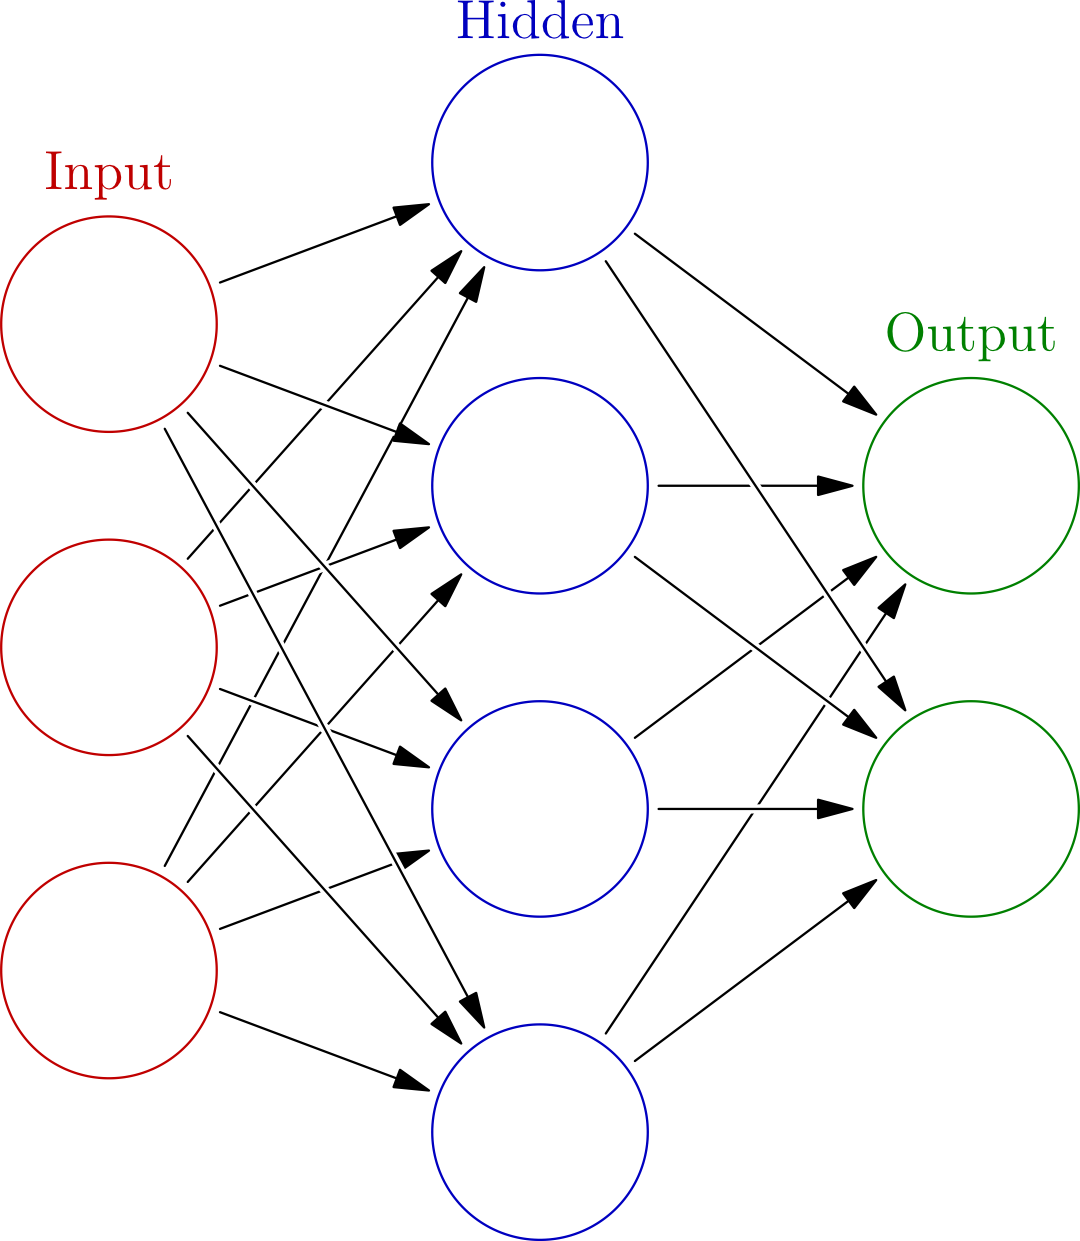
\includegraphics[height=.2\textheight]{../img/colored_neural_network.png}
  \caption{A~shallow neural network with 3 layers}
  \label{fig:shallow-neural-network}
\end{figure}

\textbf{Convolutional neural network} (CNN) is a~neural network suitable for high-dimensional inputs (e.g. a~large number of~pixels in an~image).
CNNs are frequently used in~computer vision (for identifying objects in an~image, for face detection in~photos etc.).
They are invariant to expectable transformations of~input, such as translations of~objects in~a~picture or changes in~illumination.

\textbf{Deep neural network} (DNN) is a~neural network with many hidden layers.
It can model complex non-linear relationships, e.g. in~speech, in~images, in~videos or in~board positions of~Go.

\section{Pipeline of Neural Networks}

AlphaGo employs two kinds of deep convolutional neural networks---a~\emph{policy network} (for move selection) and a~\emph{value network} (for board evaluation).
\begin{figure}[H]
  \centering
  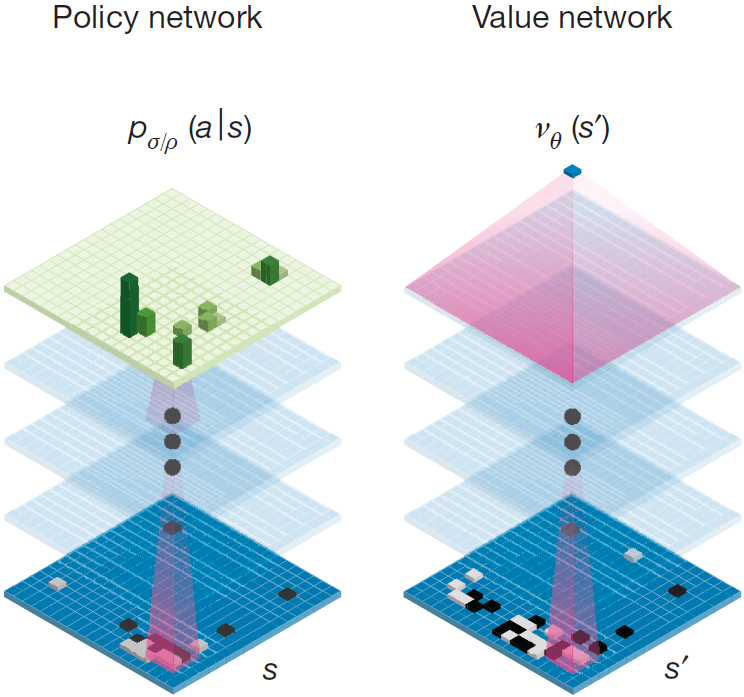
\includegraphics[width=.5\textwidth]{../img/policy_and_value_network.png}
  \captionWithCite{Comparison between policy and value network}{Silver2016mastering}
  \label{fig:policy_vs_value_nets}
\end{figure}

In the following Figure~\ref{fig:neural_nets_pipeline}, we can view the whole training process of~AlphaGo's neural networks.
\begin{figure}[H]
  \centering
  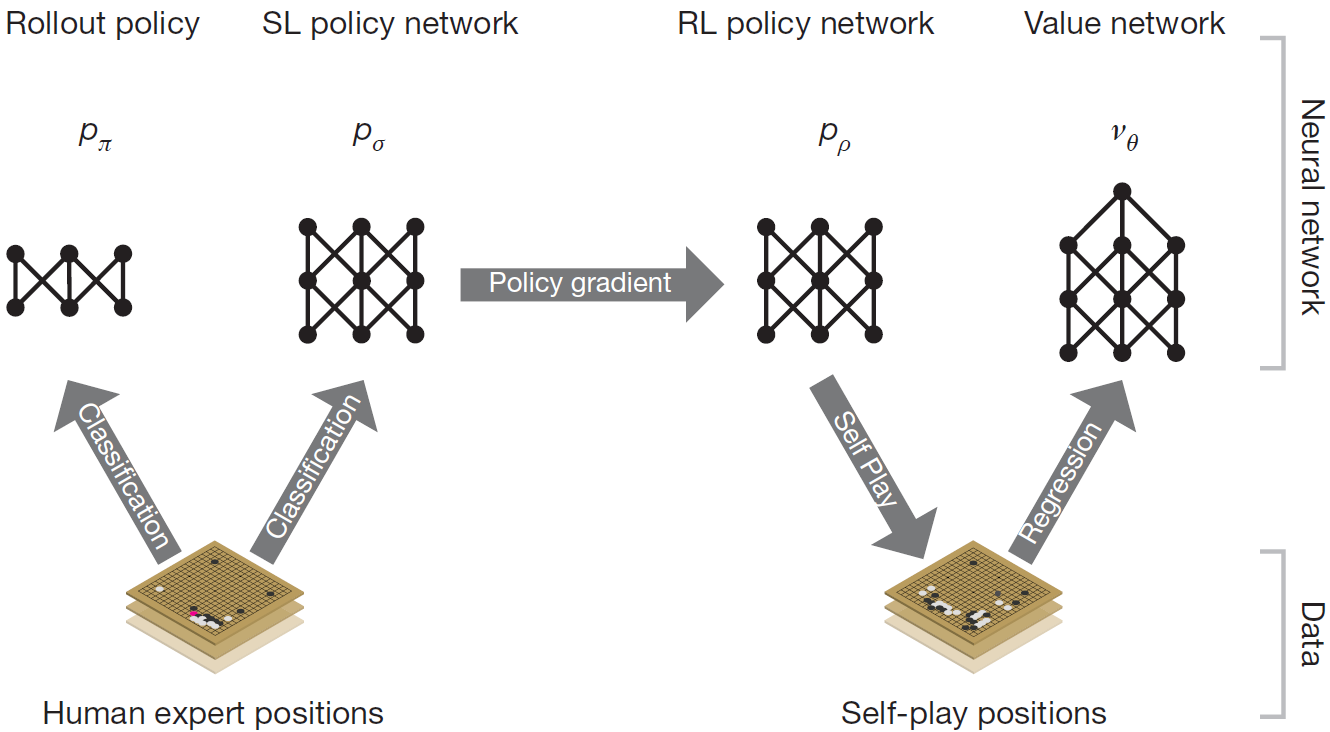
\includegraphics[width=.7\textwidth]{../img/neural_nets_pipeline.png}
  \captionWithCite{Training the neural networks of~AlphaGo: the~pipeline~and~the~architecture}{Silver2016mastering}
  \label{fig:neural_nets_pipeline}
\end{figure}

\textbf{Rollout policy} $p_\pi$ is a~CNN rapidly sampling actions during a~\emph{rollout} (a~fast-forward simulation from a~position to the end of~the game).
It predicts expert human moves much faster but less accurately than $p_\sigma$ (see below).
The output is a~probability distribution over all moves.

\textbf{Policy network} is a~CNN selecting moves.
It addresses the problem of the game-tree breadth.
There are two flavors of~these networks:
\begin{itemize}
  \item \textbf{SL policy network} $p_\sigma$ is trained by \underline{s}upervised \underline{l}earning to predict expert human moves.
  \item \textbf{RL policy network} $p_\rho$ is trained by \underline{r}einforcement \underline{l}earning to win in the~games of~self-play.
\end{itemize}

\textbf{Value network} $v_\theta$ is a~CNN evaluating board positions, so as to address the problem of the game-tree depth.
It is trained by regression to predict the outcome in~positions of~the self-played games.

\section{Main Algorithm of~AlphaGo}

Finally, the neural networks are combined with MCTS into the main algorithm.

During the play, AlphaGo simulates up to 100 possible continuations per each move by selecting the most promising actions and following them.
This way, it descends the game-tree down to a~depth given by a~parameter.
At that point, leaf nodes are evaluated in two ways:
\begin{enumerate}[(1)]
  \item using the dedicated value network $v_\theta$,
  \item simulating the self-play until the terminal positions, using the fast rollout policy $p_\pi$.
\end{enumerate}
The two are mixed into the final value of~the leaf node.

Once every simulation of a~single round is finished, all new values are backpropagated to the root, thus updating necessary variables on the way up.

For more details, consult (\cite{Silver2016mastering}) or the before-mentioned presentations.

\note{
  Main algorithm demonstrates the connection to \emph{our theme of~endgames}:
  the simulations may be viewed as ``solving endgames''.
  In particular, the $p_\pi$ rollouts somehow remind of~exhaustive search for the game value during the late stage of~the play.
  In this sense, the approaches of~AlphaGo and endgame computation bear a~striking similarity.

  On the other hand, AlphaGo performs the same simulation algorithm during the whole game:
  from an~empty board until the final move.
  Therefore, it would be imprecise to talk about ``endgame'' here.
}

\section{Playing Strength}

In order to assess the playing strength of~AlphaGo, DeepMind has organized an~internal tournament between different other Go programs,%
\footnote{\emph{CrazyStone} and \emph{Zen} are the strongest commercial programs, whereas \emph{Pachi} and \emph{Fuego} are strongest among the open-source ones.}
as well as a~duel of~AlphaGo against the European Go Champion Fan Hui.
Figure~\ref{fig:Go-tournament} displays the outcome of the tournament:

\begin{quotation} \noindent
  Each program used approximately 5 s computation time per move.
  To provide a~greater challenge to AlphaGo, some programs (pale upper bars) were given four handicap stones (that is, free moves at~the start of~every game) against all opponents.
  Programs were evaluated on an Elo scale: a~230 point gap corresponds to a~79\% probability of winning, which roughly corresponds to one amateur dan rank advantage on KGS;
  an~approximate correspondence to human ranks is also shown, horizontal lines show KGS ranks achieved online by that program.
  Games against the human European champion Fan Hui were also included;
  these games used longer time controls.
  95\% confidence intervals are shown.~(\cite{Silver2016mastering})
\end{quotation}

\begin{figure}[H]
  \centering
  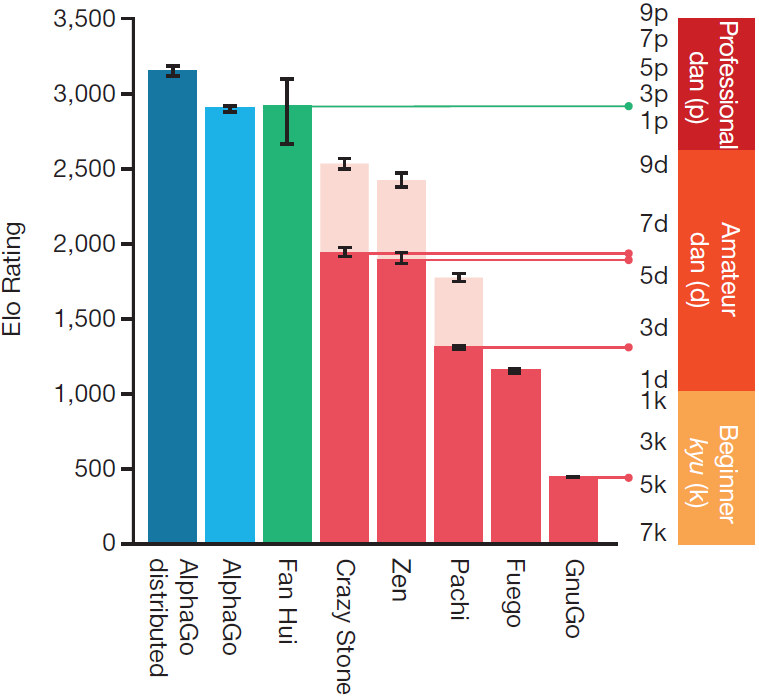
\includegraphics[width=.5\textwidth]{../img/results_of_tournament.png}
  \captionWithCite{Tournament with other programs and Fan Hui}{Silver2016mastering}
  \label{fig:Go-tournament}
\end{figure}

Here is an~official report provided by Google DeepMind%
\footnote{\href{https://deepmind.com/alpha-go.html}{https://deepmind.com/alpha-go.html}}
about AlphaGo's matches against human professionals:
\begin{quotation} \noindent
  After our program AlphaGo won 5--0 in a~formal match on~October 2015, against the reigning 3-times European Champion, Fan Hui, becoming the first program to ever beat a~professional Go player in an~even game;
  AlphaGo then went on to complete its ultimate challenge.

  In March 2016 AlphaGo won 4--1 against the legendary Lee Sedol, the top Go player in the world over the past decade.
  The matches were held at the Four Seasons Hotel, Seoul, South Korea on March 9\textsuperscript{th}, 10\textsuperscript{th}, 12\textsuperscript{th}, 13\textsuperscript{th} and 15\textsuperscript{th} and livestreamed on DeepMind’s YouTube channel as well as broadcast on TV throughout Asia through Korea’s Baduk TV, as well as in China, Japan, and elsewhere.

  They were played under Chinese rules with a~komi of~$7.5$ (the compensation points the player who goes second receives at~the end of~the match).
  Each player received two hours per match with three lots of 60-second byoyomi (countdown periods after they have finished their allotted time).
\end{quotation}

Following from this, computers seem to have reached the ``superhuman'' level of~expertise and they now appear to be superior to humans in~the game of~Go.
